\chapter{Results}
\epigraph{The first law of thermodynamics says that work cannot be destroyed. We who use computers know better.}{A frustrated Ph.D. candidate}

Applying the procedure summarized in the previous chapter resulted in the discovery of four new periodic orbits. We will discuss some of their properties below, before moving on to analyze the behavior of the shortest period orbit. We find that the application of linear stability analysis works as expected, and find behaviors that are suggestive of bifurcations under varying $L_z$.   
\section{The Gang of Four}

The four new \ecs\ are periodic orbits, P85, P60, P32 and P8 have been found. We call these orbits the `Gang of Four', and label them by the integer part of their period since experience shows that the period of an orbit uniquely identifies the orbit.\footnote{We generally assume that if two solutions have differing periods, they are distinct, which may seem reasonable - but holes in such a simple criterion are evident almost immediately. For example, two `distinct' orbits with periods $T_1$ and $T_2$ may in fact be the same orbit, with period $|T_2-T_1|$, that has simply repeated more times for one orbit than for the other. This hole can be plugged by any number of methods, most easiest by simply calculating $||\Vector{u}_1(t) - \Vector{u}_2||$ over the entire period. If the norm is never small, then the orbits are distinct. }.  P85 and P60 are in the fully symmetric subspace, while P32 is in $S_x$ with a streamwise relative velocity of $v_x = 0.5$ and P8 is in $S_z$, with a spanwise relative velocity of $v_z = 2.29\times 10^{-7}$. This seems rather low, but is above the noise threshold of {\tt Channelflow},\footnote{John Gibson, private communication.} and is required for the NKH solver be able to converge to a solution, so we feel justified in stating that P8 has a nonzero $v_z$. We were unable to find any \ecs\ in the asymmetric subspace. Other properties of the Gang of Four, including their largest Floquet exponents $\lambda_{\textrm{max}}$ and number of unstable Floquet exponents $\lambda_{\textrm{unstable}}$ (\refSec{sec:LSA}), as well as their mean dissipation and energy input ($\bar{D}/\bar{I}$) (\refSec{sec:DI}) at  $\ReN = 400$, in the Hamilton-Kim-Waleffe (HKW) cell\rf{Hamilton1995} with $(L_x,L_z) = (5.51157, 3.76239)$, and grid discretization $(N_x,N_y,N_z)= (48,33,48)$  are summarized in \refTab{tab:summary}. 

\begin{table}[h!]
\caption{A summary of some relevant information regarding the Gang of Four at $\ReN = 400$, in a periodic cell with $(L_x,L_z) = (5.51157, 3.76239)$, and grid discretization $(N_x,N_y,N_z)= (48,33,48)$. The symmetry isotropy subgroup of each orbit is also provided.}\label{tab:summary}
\begin{center}
\begin{tabular}{r   c  c  c  c  c  c  c  l }
\toprule
Label & $T$ & $v_x$ & $v_z$ &  $\lambda_{\textrm{max}}$ & $\#\ \lambda_{\textrm{unstable}}$ & $\bar{D}/\bar{I}$&  Symmetry \\
\midrule
\midrule
P85 & 85.50 & 0 & 0 & 0.0427 & 6 &1.85 & S\\
P60 & 60.86 & 0 & 0 &  0.032749 & 10 & 2.08 & S\\
P32 & 32.00 & 0.5 & 0 &  $0.0200 + 0.0982 \mathbbm{i}$ & 7& 1.98 &$S_x$\\
P8 & 8.32 & 0 & $2.29\times 10^{-7}$ & $0.0998 - 0.2605 \mathbbm{i}$ &20& 4.00& $S_z$\\
\bottomrule
\end{tabular}
\end{center}
\end{table}

\subsection{Visualizations}   
In order to gain a better understanding of the Gang of Four, it can use useful to visualize the flow state. Visualizing the behavior of fluids is in itself a time-honored discipline, especially when CFD is involved,\footnote{As the old joke goes, CFD really stands for {\bf C}olorful {\bf F}luid {\bf D}ynamics.} and well chosen visualization schemes can be, in and of themselves, an excellent tool for interpreting and analyzing data. Here, we use two main visualization methods.
\subsubsection{Orthographic Projection}
\refFigsss{fig:p85}{fig:p60}{fig:p32}{fig:p8} are all examples of the first visualization method -- the {\bf orthographic projection} (OP)\rf{Gibson2008}, which is handily provided by the {\tt Channelflow} utility functions {\tt plotbox} and {\tt movieframes} for diagrams and movies respectively. The OP is constructed by piecing together several representative 2D slices of the state's velocity field -- each of the periodic boundaries, and the mid-plane, and is colored to represent the magnitude and direction of streamwise velocity -- redness corresponds to the magnitude of positive streamwise flow, while blueness represents the magnitude of negative streamwise flow.\\

The OP allows us to visually interrogate the structure of the state, which can be extremely useful -- for example, it is clear purely from visual interrogation that \refFig{fig:p8} is less ordered than \refFig{fig:p85}. In this case, each of these figures show only the perturbation field,\footnote{That is, the laminar flow has been subtracted before the visualization is made.} and animations of their evolution through a period are available online.\footnote{See the caption of the relevant orbit for URLs.} The fact that P85 and P60 are in the fully symmetric subspace is reflected in their extreme symmetry under both rotations about the spanwise axis and reflections about the streamwise axis. However, the midplane streaks of P60 are of lower energy than those of P85. Despite the fact that P32 has streamwise broken symmetry, its OP shows that it has streak features that are remarkably reminiscent of those found in P85 and P60. Applying the {\tt Channelflow} utility function {\tt findsymmetries} in its verbose mode to P32 reveals that $\sigma \Vector{u} - \Vector{u} = O(10^{-2})$ for $\sigma = \sigma_z \tau_x$. While this is insufficient to be categorized as an invariant symmetry,\footnote{The default creterion used by {\tt findsymmetries} is that $\sigma$ is an invariant symmetry if $\sigma\Vector{u} - \Vector{u}$ is satisfied to at least $10^{-6}$. I see no reason to change that.} it should be noted that most unsatisfied symmetries have  $\sigma\Vector{u} - \Vector{u} = O(1)$, so P32 only slightly breaks streamwise symmetry.\\

P8 has no midplane streaks, but has a prominent roll structure and most importantly, has a period that is to an order of magnitude lower than the other orbits. This is very useful, since the Arnoldi iteration (which is central to almost all the analysis methods used here) scales linearly with time, so the analysis of P8 takes an order of magnitude less time.\footnote{For example, a single iteration of \refAlg{alg:parCont} takes about 2 hours for P8, which allowed us to collect the data presented in \refFig{fig:LZBif} in about a week. The same process would have taken more than a month for P32, and several for P60 and P85.}

\begin{figure}[h!]
\centerline{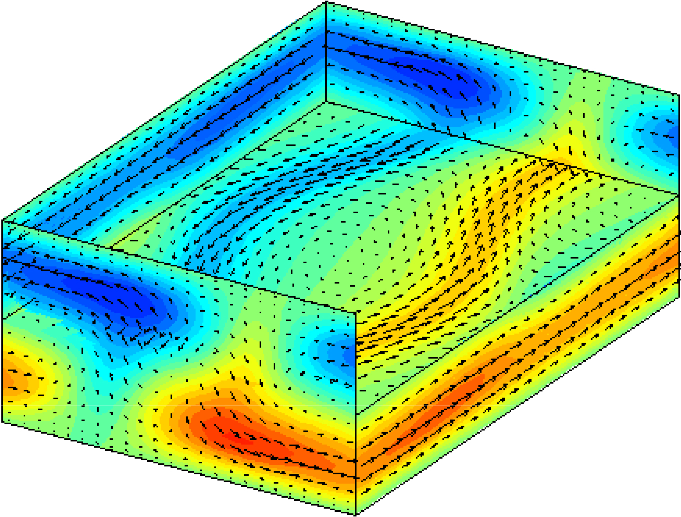
\includegraphics[scale = .9]{p85noBase.pdf}}
\caption{Orthographic projection of P85. P85 is a fully symmetric orbit in the HKW cell, with period 85.50 at $\ReN=400$. Note the extreme symmetry of the prominent streaks visible in the mid-plane. The velocity field pictured here is the turbulent perturbation only; the laminar flow has been subtracted away.{ Animation available at {\tt http://goo.gl/hxRp8E}}}\label{fig:p85}
\end{figure}

\begin{figure}
\centerline{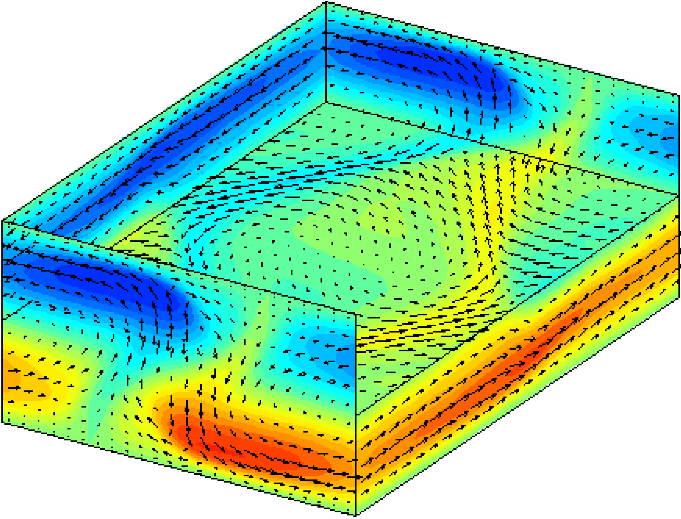
\includegraphics[width=\textwidth]{p60noBase.pdf}}
\caption{Orthographic projection of P60. P60 is another fully symmetric orbit  in the HKW cell, with period 60.86 at $\ReN = 400$.  The velocity field pictured here is the turbulent perturbation only; the laminar flow has been subtracted away.{ Animation available at {\tt http://goo.gl/4fQalm}}}\label{fig:p60}
\end{figure}


\begin{figure}
\centerline{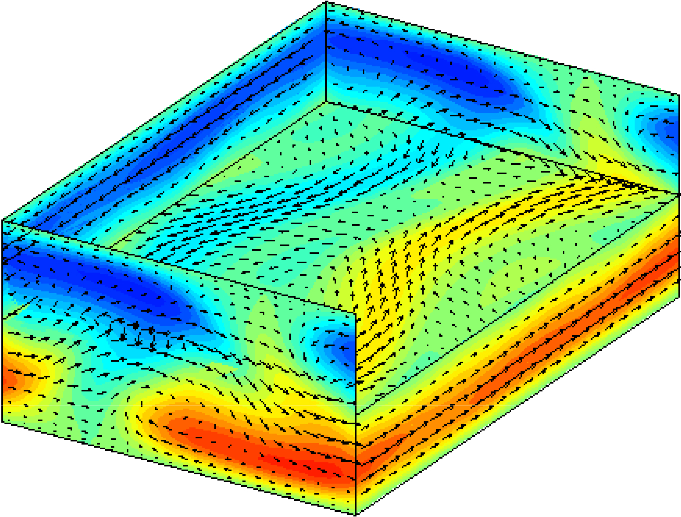
\includegraphics[width=\textwidth]{p32noBase.pdf}}
\caption{Orthographic projection of P32. P32 is a streamwise asymmetric periodic orbit fixed by the symmetry group $S_z$. $S_z$  is functionally a mirror symmetry about the streamwise axis. The velocity field pictured here is the turbulent perturbation only; the laminar flow has been subtracted away. Animation available at {\tt http://goo.gl/E8wRLm}}\label{fig:p32}
\end{figure}


\begin{figure}
\centerline{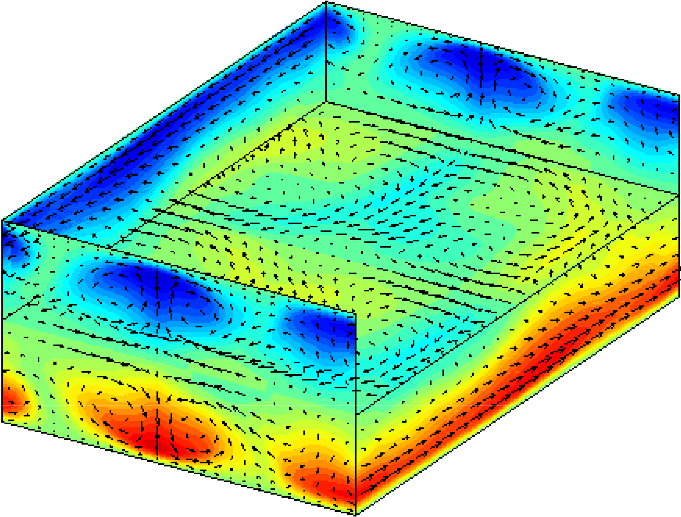
\includegraphics[width=\textwidth]{p8noBase.pdf}}
\caption{Orthographic projection of P8. P8 is a spanwise asymmetric periodic orbit fixed by the symmetry group $S_x$. $S_x$ is functionally a rotation by $\pi$ about the spanwise axis. The velocity field pictured here is the turbulent perturbation only; the laminar flow has been subtracted away. Animation available at {\tt http://goo.gl/uTDrLw}}\label{fig:p8}
\end{figure}

\clearpage
\subsubsection{State Space Projection}
If more quantitative analyses are desired, however, the OP cannot deliver. For this reason, we use a second, more useful visualization method - the state space projection\rf{Gibson2008}, which is provided by the {\tt Channelflow} utility functions {\tt projectfields} and {\tt projectseries} for single points and trajectories respectively. Since we think of our trajectories as living in a high dimensional state space, it is natural to imagine projecting these trajectories onto lower dimensional manifolds, in much the same way that we render 3D objects in a 2D drawing. If we have a set of $k$ basis vectors $\Vector{q}_k$ that are orthonormal and span a subspace $\mathfrak{V}_k \subset \mathfrak{V}$ of dimension $k$, then the projection of a vector $\Vector{v} \in \mathfrak{V}$ onto $\mathfrak{V}_k$ is defined 
\begin{equation}
\Vector{v}_k = \sum{i = 1}{k}{c_i \Vector{q}_i},
\end{equation}
where $c_i = \Vector{v} \cdot \Vector{q}_i$. Projecting the trajectory becomes extremely useful when $k$ is either 2 or 3, since we can then visualize the $n$-dimensional trajectory as a 2 or 3 dimensional projection instead. We do lose information in making this projection, but gain the ability to visualize some part of the trajectory. \\
\begin{figure}[h]
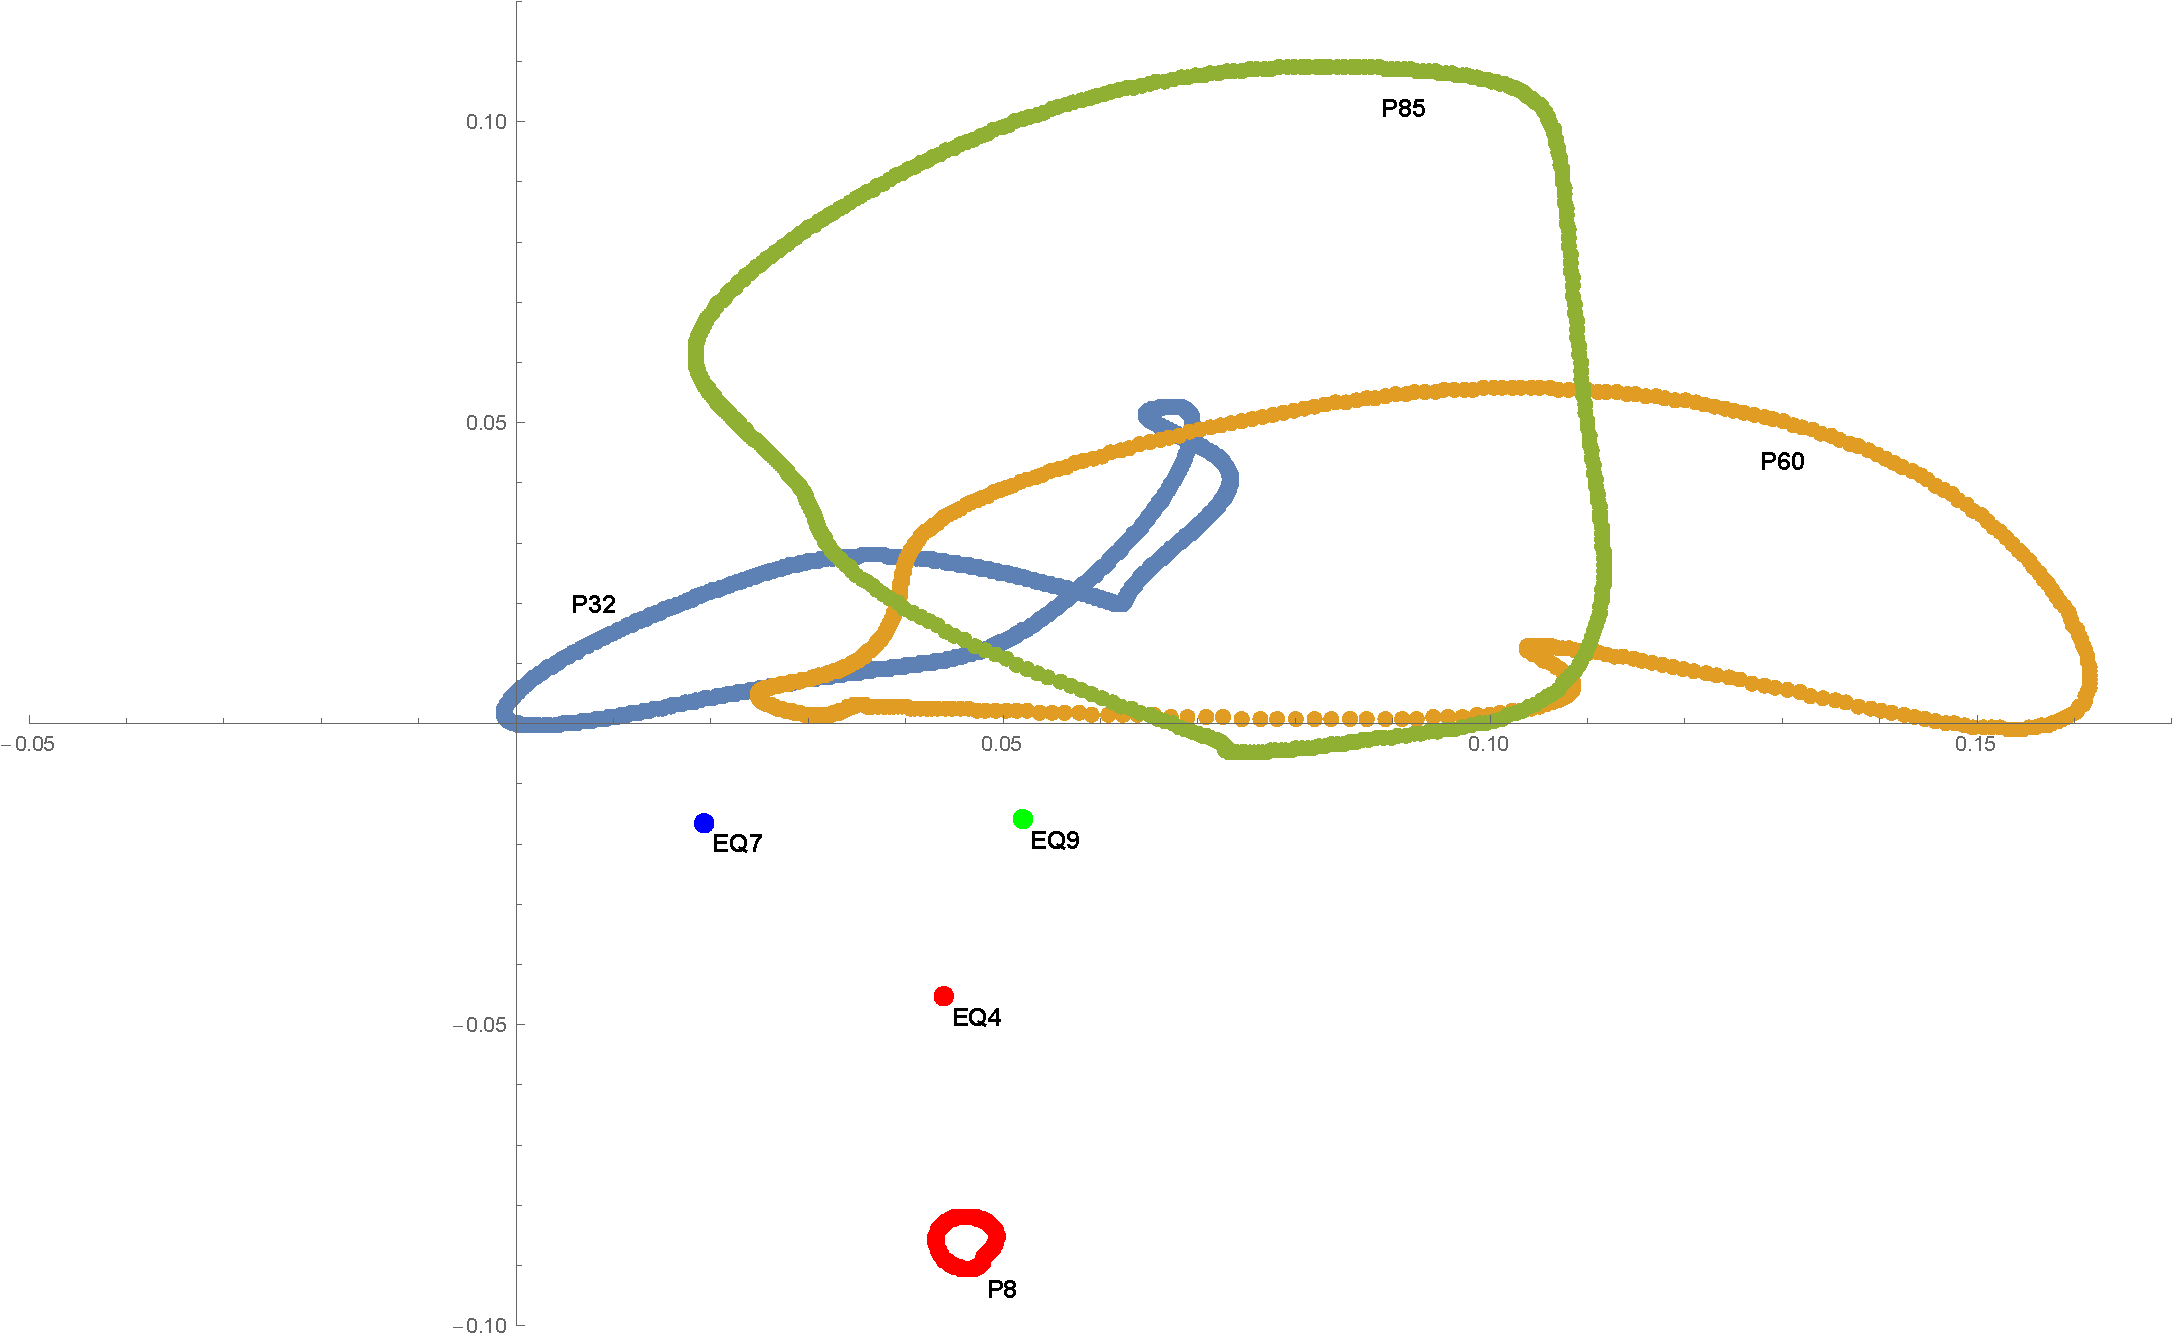
\includegraphics[width=\textwidth]{PeriodicOrbitPO412}
\caption{2D state space projection of the Gang of Four and some reference equilibria from Halcrow\rf{Halcrow2008}. The basis vectors for the projection were constructed by orthonormalizing the initial states of each of the periodic orbits using the Gram-Schmidt procedure.}\label{fig:POStateSpace}
\end{figure}
\clearpage Projecting the four periodic orbits in \refFigRange{fig:p85}{fig:p8} onto a basis constructed by orthonormalizing the initial conditions of each orbit using the Gram-Schmidt procedure results in the state space projections in \refFig{fig:POStateSpace}. Projecting onto this basis produces a 4D state space projection, from which we can take 2D slices (of which there are 6), or 3D slices (of which there are 4). Equilibria found by Halcrow\rf{Halcrow2008}, which are fully symmetric are included for reference.  Notice that the P8 orbit is separated by the equilibria from P85, P60 and P32, a feature that holds true in the other 5 2D projections. Notice also that P32 remains close to its symmetric brethren in this projection -- we believe this is a result of P32 having only slightly broken its streamwise symmetry. \\

One technical  issue with the state space projection method, however, is that a state must be {\bf congruent} to a basis to be projected onto it - that is, both the box length and grid discretization must be the same for both the state and the projection basis. Many previous investigations\rf{Halcrow2008,Gibson2008} have important results in the Wallefe '03 (W03) cell, where $(L_x,L_z) = (5.51157,2.51327)$. In order to compare with these results, we attempted to use \refAlg{alg:parCont} to continue the four periodic orbits into the W03 cell. This led us to the next important result.

\section{Spanwise Continuation}

When \refAlg{alg:parCont} was used to continue P8 down to the W03 cell, the data presented in \refFig{fig:LZBif} was produced.  Initially, the continuation algorithm decreases $L_z$ and increases $T$ along the {\bf upper branch}, but at $L_z$ in the interval $[2.8087, 2.8096]$, the algorithm reverses itself at the {\bf first turning point} $\mathfrak{Z}_1$, decreasing $T$ and increasing $L_z$ along the {\bf transition branch}. This continues until it encounters the {\bf second turning point} $\mathfrak{Z}_2$ at  $L_z$ in the interval $[2.6140,2.6157]$, at which point the algorithm resumes decreasing $L_z$ and increasing $T$ along the {\bf lower branch}.\\

 so  the existence of multiple, distinct orbits for $\mathfrak{Z}_1 \leq L_z \leq \mathfrak{Z}_2$ hints at a bifurcation.
\begin{figure}[t]
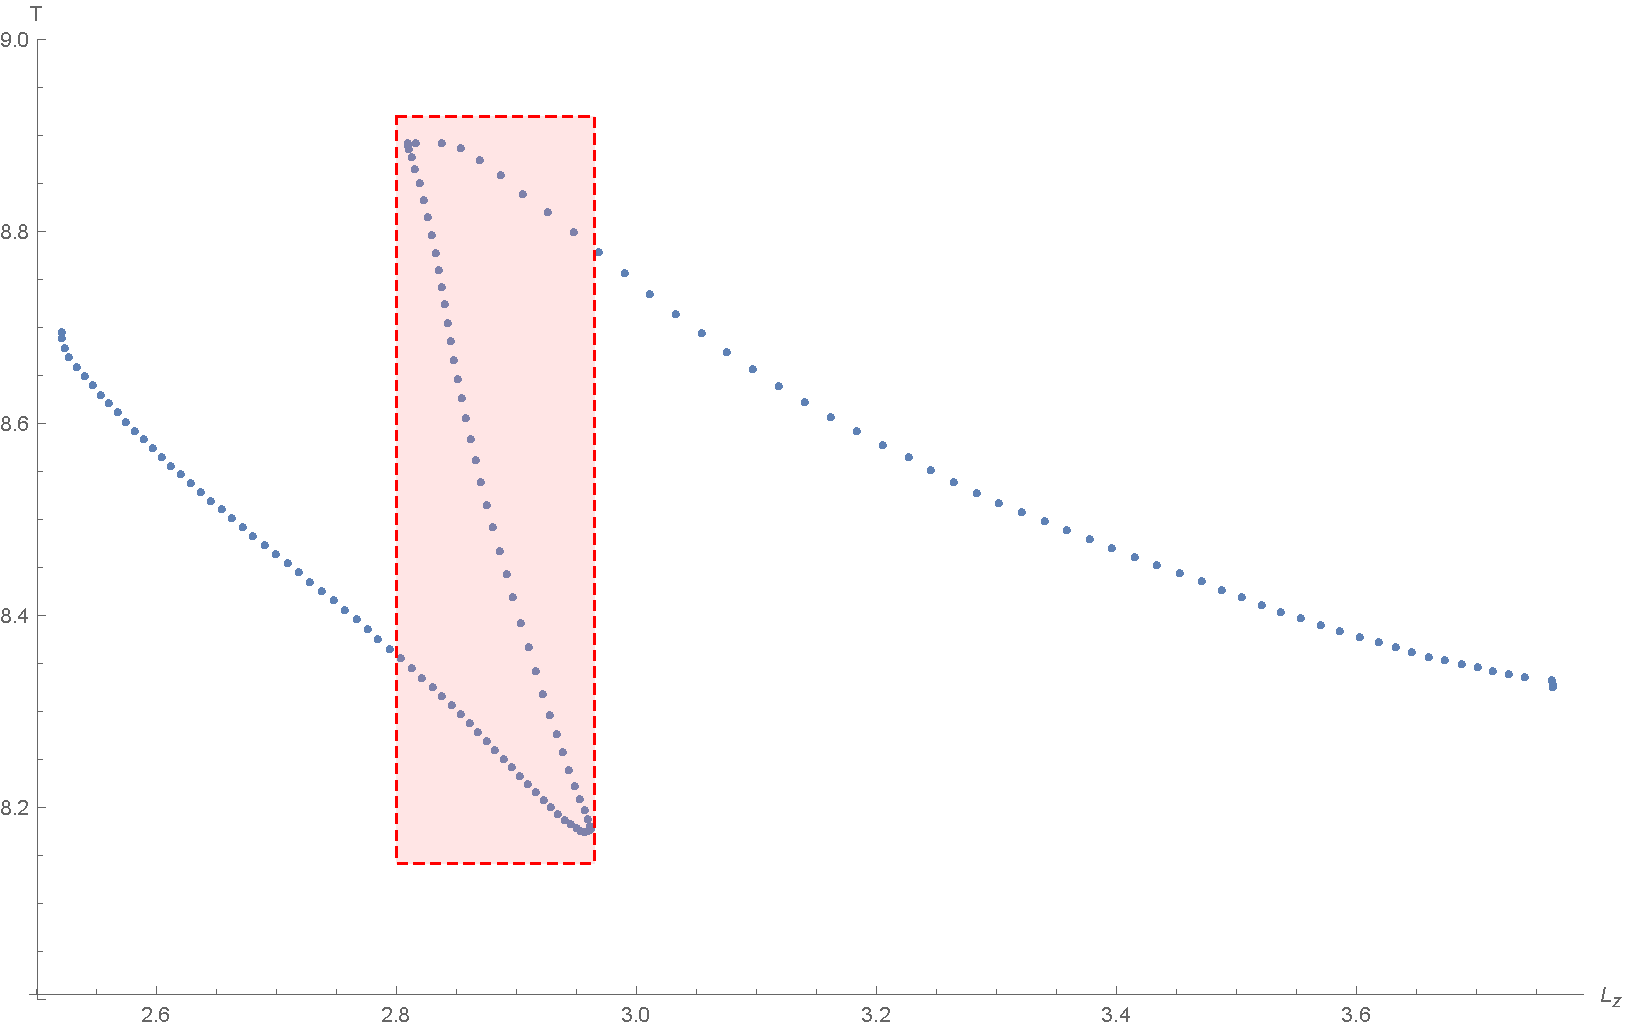
\includegraphics[width=\textwidth]{TLzBD}
\caption{Period as a function of spanwise cell length for P8. The {upper branch} (blue circles), the {transition branch} (green diamonds), the { lower branch} (orange rectangles) and the two turning points (red, dashed circle and purple, solid circle) are displayed. Within the marked rectangular region, multiple distinct solutions exist for the same cell length, hinting at a bifurcation.}\label{fig:LZBif}
\end{figure}
\begin{figure}[t]
\includegraphics[width=\textwidth]{phasePortraitTransition}
\caption{Phase portrait of the Van Der Pol oscillator\rf{VanderPol1926} and its Hopf bifurcation, with trajectories in white. (a) For negative values of the bifurcation parameter, the single periodic orbit is unstable, so an initial condition that begins near the orbit spirals away from it. (b) When the bifurcation parameter is zero, there is no periodic orbit. (c) For positive values of the bifurcation parameter, the periodic orbit is stable, and initial conditions are attracted into the orbit.}\label{fig:phasePortrait}
\end{figure}
However, \refAlg{alg:parCont} relaxes the convergence criterion to $10^{-10}$ to speed up the parametric continuation process, and as a result, may have found artificial solutions, so we verified the existence of multiple distinct solutions for $L_z = 2.925$ and $(N_x,N_y,N_z) = (62,53,62)$ to $10^{-13}$. It is important to note that this in and of itself does not necessarily prove that a bifurcation exists -- for example, the continuation algorithm may have simply found \emph{another} periodic orbit's trajectory and hopped onto that. When a bifurcation occurs, the qualitative behavior of solutions pre and post-bifurcation tend to be markedly different. For low-dimensional systems, this is easy to evaluate, since one can visually identify changes in the phase space, as in \refFig{fig:phasePortrait}. For higher-dimensional systems, such an approach is not feasible. 

\subsection{Linear Stability Analysis}\label{sec:LSA}

Instead, we can turn to {\bf linear stability analysis}. If $\Vector{u}$ is a periodic orbit with period $T$, then for a small perturbation ${\bf \textrm{d}}\Vector{u}$, 
\begin{equation}\label{eq:linearStable}
 f_T(\Vector{u} + {\bf \textrm{d}}\Vector{u}) - \Vector{u} =  f_T(\Vector{u}) - \Vector{u} + \mathbb{J}_{T,\Vector{u}}{\bf \textrm{d}}\Vector{u} =  \mathbb{J}_{T,\Vector{u}}{\bf \textrm{d}}\Vector{u},
\end{equation} 
where $ \mathbb{J}_{T,\Vector{u}}$ is the Jacobian of the Navier-Stokes forward-time map evaluated at $\Vector{u}$. The stability of the orbit is determined by how  ${\bf \textrm{d}}\Vector{u}$ changes over time - if it shrinks, then the orbit is stable, but if it grows, it is unstable. Writing  ${\bf \textrm{d}}\Vector{u}$ as a linear combination of the eigenvectors $\Vector{w}_i$ of  $ \mathbb{J}_{T,\Vector{u}}$, the right-hand side of \eqref{eq:linearStable} becomes
\begin{equation}\label{eq:oneOrbit}
 \mathbb{J}_{T,\Vector{u}}{\bf \textrm{d}}\Vector{u} =  \mathbb{J}_{T,\Vector{u}}\sum{i = 1}{n}{c_i\Vector{w}_i} = \sum{i = 1}{n}{c_i\lambda_i\Vector{w}_i},
\end{equation}  
where $\lambda_i$ is the eigenvalue of the eigenvector $\Vector{w}_i$, known as the {\bf Floquet exponent}. Its real part measures the exponential rate of decay or growth of perturbations along $\Vector{w}_i$.\footnote{The real part is known as the {\bf Lyapunov exponent}. The imaginary part contributes only to the oscillatory behavior.}   From this definition, it is clear that the periodic orbit can only be stable against infinitesimal perturbations if $\textrm{Re}[\lambda_i]  \leq 0~\forall~i$, and unstable otherwise. The eigenvalues for the Navier-Stokes forward-time map can be calculated by \refAlg{alg:Arnoldi}. The eigenvalues of P8 in the HKW cell at $\ReN=400$ are shown in \refFig{fig:P8Eigenvals}. Note that many of the eigenvalues come in conjugate pairs. Since there are some eigenvalues with positive real parts, the periodic orbit is unstable, as expected. Note that since the Jacobian likely has full rank, and likely also has no repeating nonzero eigenvalues, there are several orders of magnitude more stable eigenvalues than there are unstable. Luckily, the Arnoldi iteration finds the larger eigenvalues first, so we can find all the unstable eigenvalues, whereas only the weakly stable eigenvalues are calculated.\\

\begin{figure}[h]
\includegraphics[width=\textwidth]{P8Eigenvals}
\caption{All 20 unstable eigenvalues, and the 30 largest stable or marginal $(|\lambda| = 0)$ eigenvalues of P8, in the HKW cell at $\ReN=400$. }\label{fig:P8Eigenvals}
\end{figure}

In general, we would expect that as the control parameter changes, the Lyapunov exponents would also. In particular, if a change in the control parameter resulted in the Lyapunov exponent changing sign, the qualitative behavior of the periodic orbit would change, resulting in a bifurcation. Applying the Arnoldi iteration to the states near the turning points of \refFig{fig:LZBif} results in \refFig{fig:P8FirstBifurcation} and \refFig{fig:P8SecondBifurcation}. \\
\clearpage
 \refFig{fig:P8FirstBifurcation} has a set of eigenvalues change in stability at $L_z \in [2.81509, 2.81857]$, which is close to predicted values of $\mathfrak{Z}_1$. \refFig{fig:P8SecondBifurcation} has two sets of eigenvalues that change in stability at $L_Z \in  [2.96122,2.96137]$ and $L_z \in [ 2.96142,2.9615]$ respectively. The latter interval is consistent with the predicted valued of $\mathfrak{Z}_2$. Since the changes in eigenvalue stability are reasonably consistent with turning point data from \refFig{fig:LZBif}, it seems likely that these turning points do in fact correspond to bifurcations. Qualitative differences between the upper and transition branch are also apparent from observations of movies of the periodic orbit.\footnote{Available at {\tt https://youtu.be/JDzQfjx5Cmg}} From the video, it appears that the upper branch has more energy concentrated in the streaks than the transition branch, which in turn appears to have more energy in the mid-plane. \\

\begin{figure}[t]
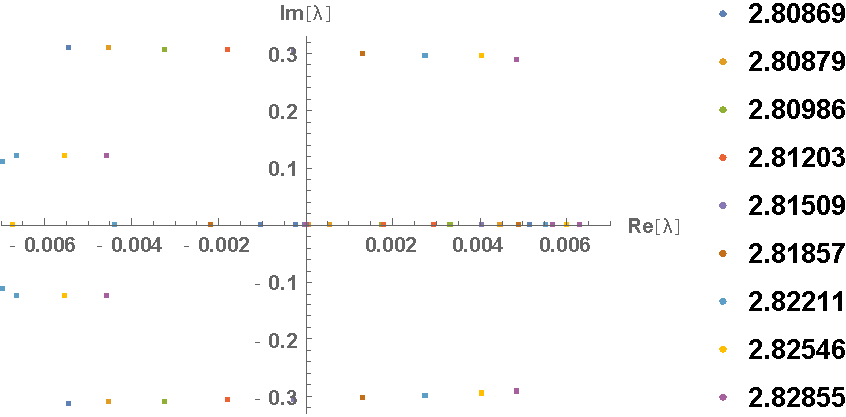
\includegraphics[width=\textwidth]{P8FirstBifurcation}
\caption{Eigenvalues of P8 as a function of $L_z$ at the first turning point. When the real part of the eigenvalue switches sign, the associated eigenvector switches stability. Therefore, the line of eigenvalues with imaginary part  $\approx \pm 0.3$ are of special interest.}\label{fig:P8FirstBifurcation}
\end{figure}


\begin{figure}[h]
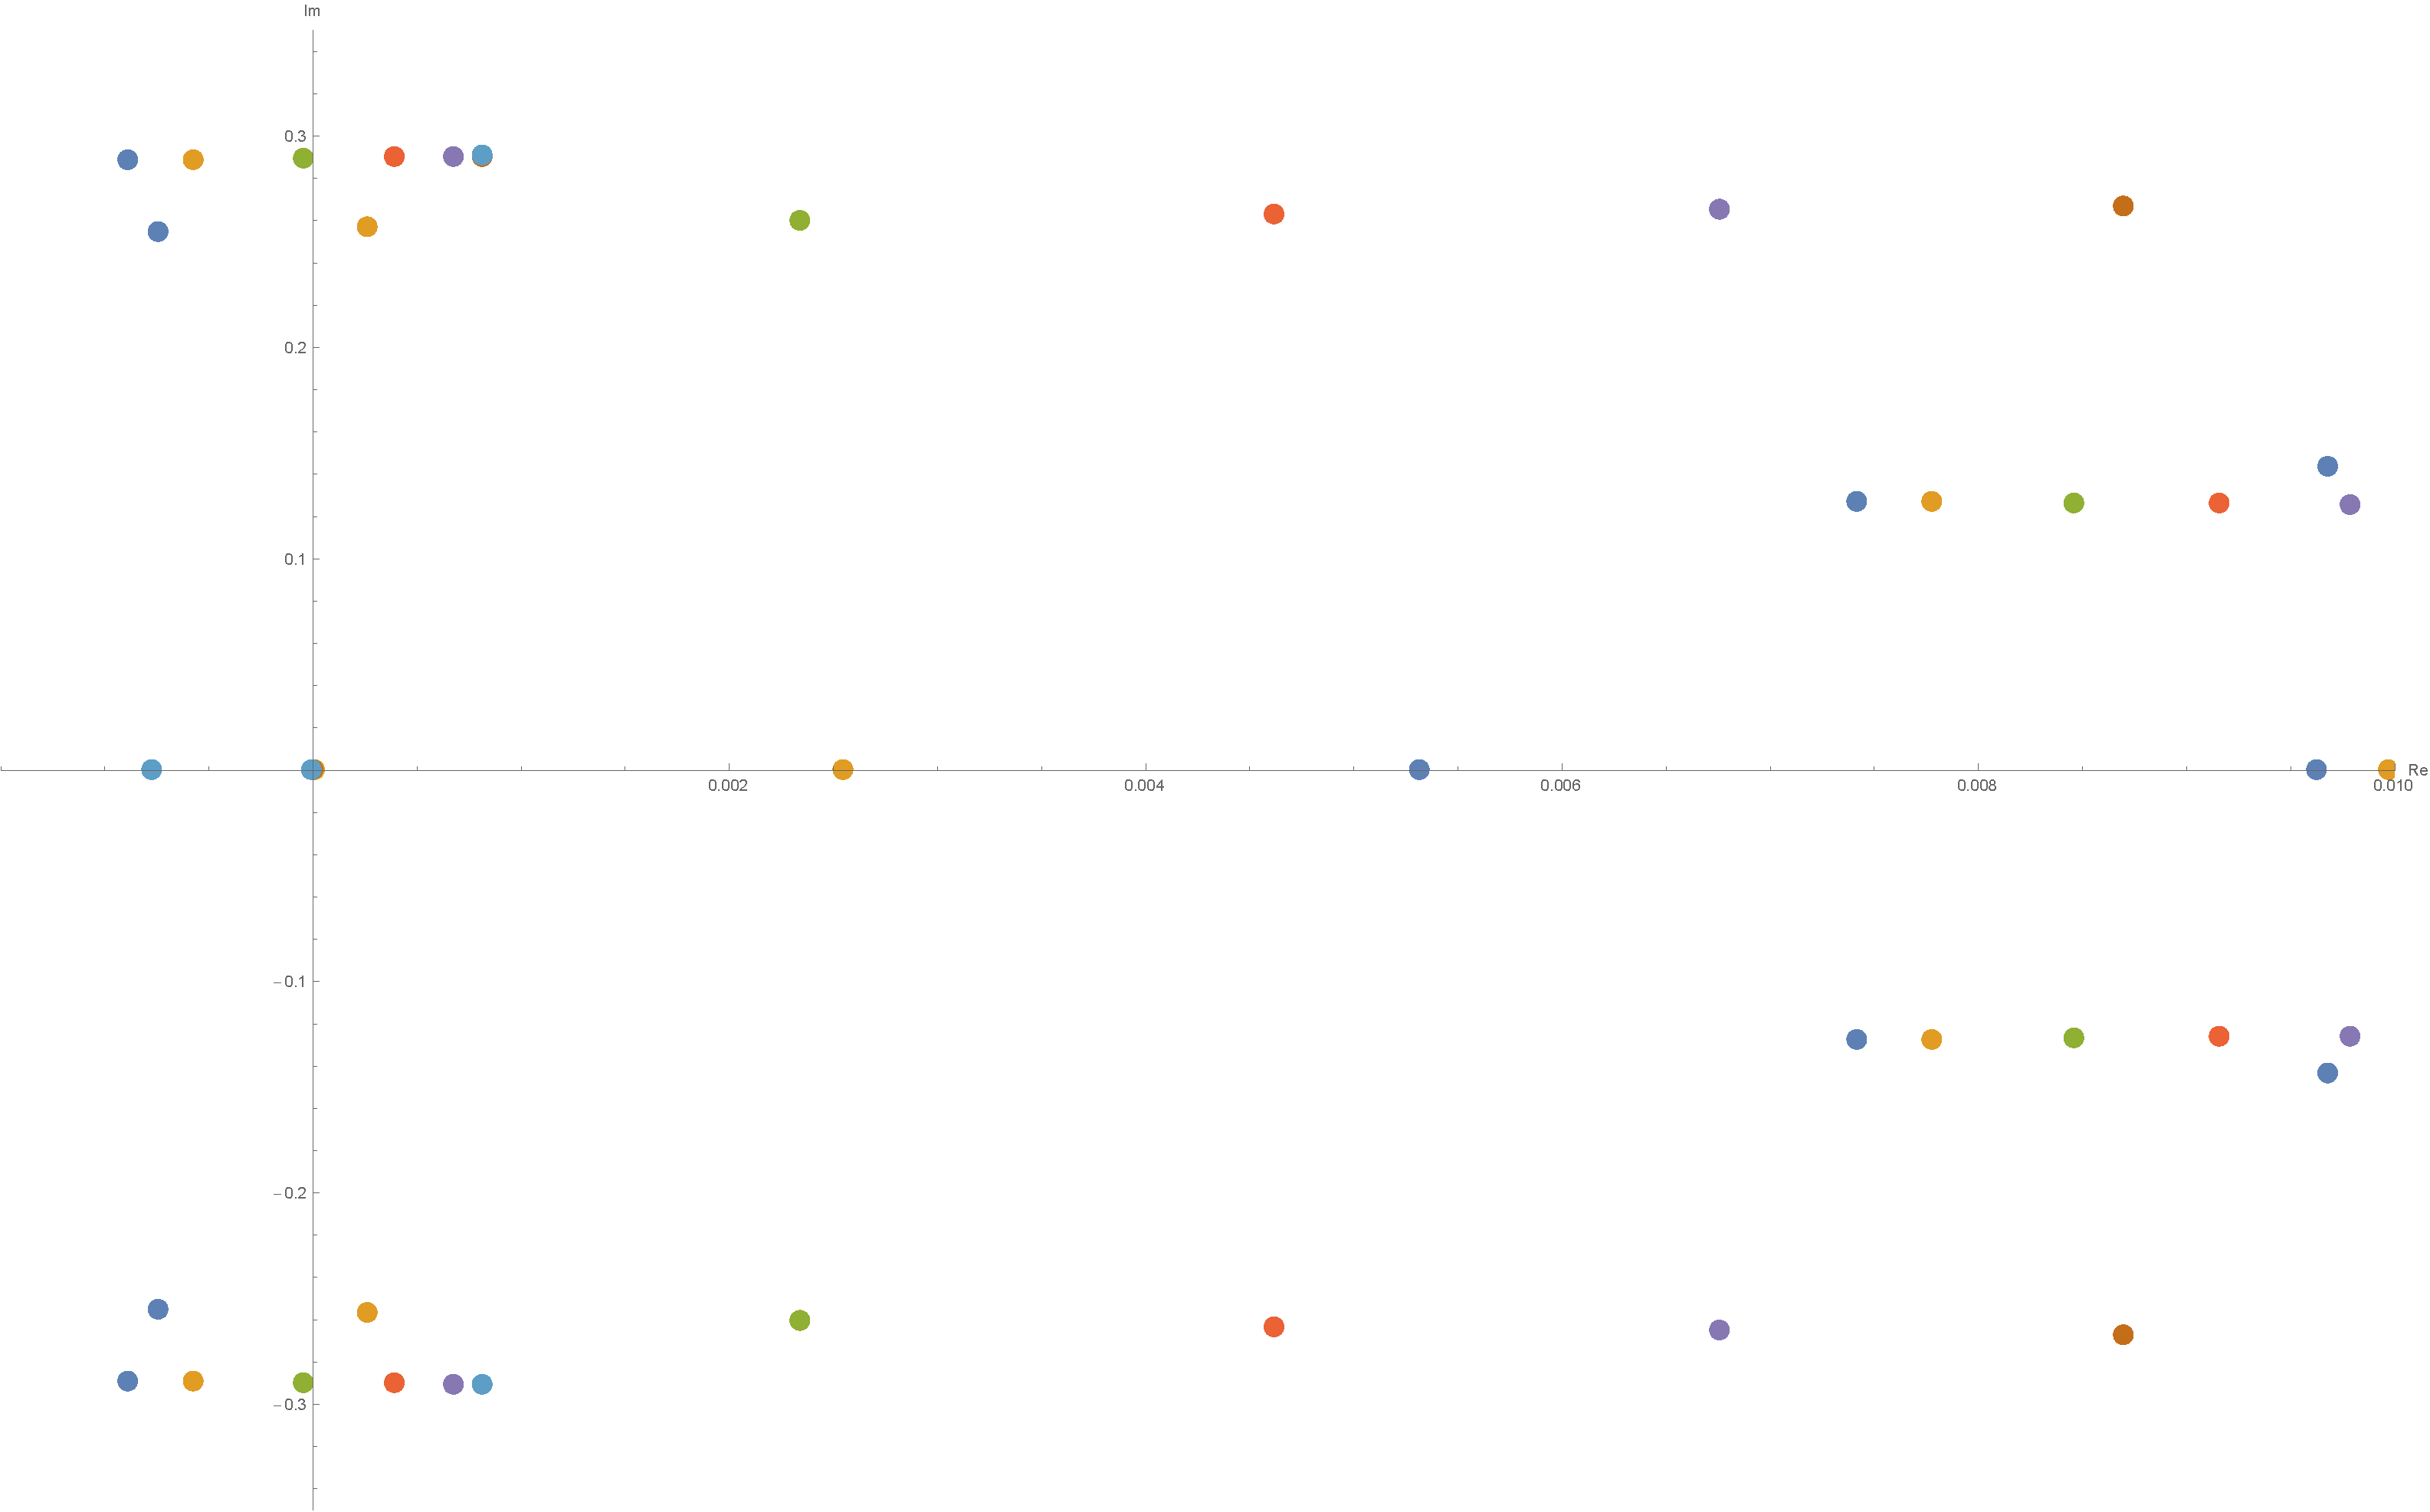
\includegraphics[width=\textwidth]{P8SecondBifurcation}
\caption{Eigenvalues of P8 as a function of $L_z$ at the second turning point. Here, two sets of eigenvalues have real parts that switch signs. }\label{fig:P8SecondBifurcation}
\end{figure}

\subsection{Return of the State Space}

Having used linear stability analysis to find the unstable eigenvectors, we can use the state space projection to visualize the effect of a slight perturbation along one of these eigenvectors, as shown in \refFig{fig:p8E1}. Here, we perturb along the most unstable eigenvector $P8E1$, which has eigenvalue $0.0998 - 0.2605 i$. Now \refFig{fig:p8E1} is noisy, and difficult to analyze. To deal with this, we can construct the {\bf Poinca\'e section} of the trajectory. The Poincar\'e section of a $k$ dimensional trajectory is constructed by keeping track of where the trajectory crosses a $k-1$ dimensional surface. The Poincar\'e section for  $P8E1$, displayed in \refFig{fig:E1Poincare} displays the qualitative behavior we would expect for a complex eigenvalue - the real part is positive and the perturbation grows, the imaginary part is nonzero, and the perturbation spirals around the initial position. Even though the Floquet exponent is only valid locally, we can still see that it approximately predicts the behavior of the trajectory - from the imaginary part of the eigenvalue, we can see that it ought to take approximately 25 time units for a full rotation in the Poincar\'e section. \refFig{fig:E1Poincare} suggests that approximately 5 orbits have taken place for a full rotation in the Poincar\'e section, each with periods that are approximately 8 time units. This does not agree exactly,\footnote{Or very well at all, especially since we've just come from having residuals on the order of $10^{-14}$.} but one must remember that the Floquet exponents are a \emph{local} model of the orbit, and naturally become less precise the more the perturbation grows.\footnote{As a matter of fact, the pictured spiral is the last spiral the Poincar\'e section trajectory executes, though the trajectory in the full space continues to look qualitatively similar to the original orbit for a long time.}   


\begin{figure}[h!]
\centerline{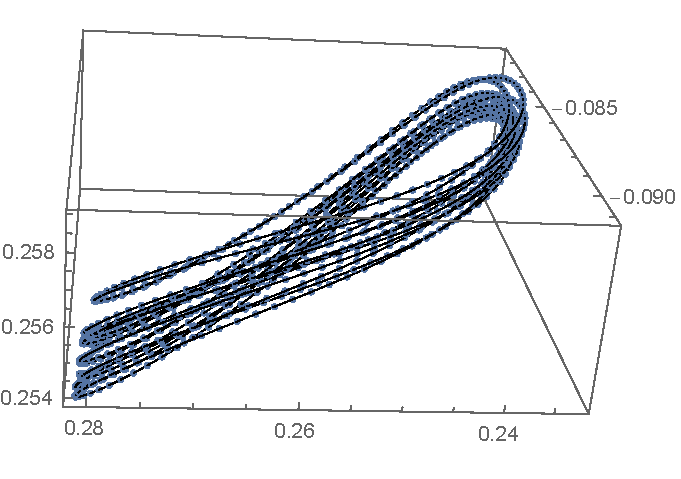
\includegraphics[scale=1]{E1Perturb}}
\caption{The trajectory of a slight perturbation along the most unstable eigenvector, projected onto a difference 2D slice of the same basis as in \refFig{fig:POStateSpace}. Notice that it keeps the general shape of the orbit that spawned it, at least for short time spans.}\label{fig:p8E1}
\end{figure}

\begin{figure}[h!]
\centerline{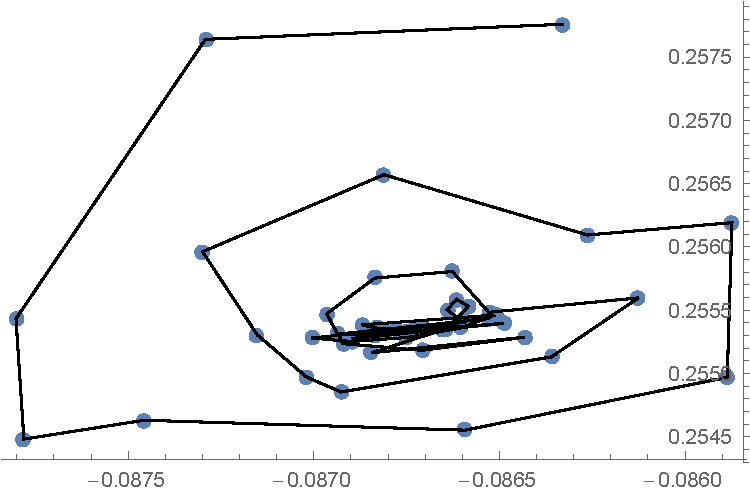
\includegraphics[scale = 0.9]{E1Poincare}}
\caption{Poincar\'e section of \refFig{fig:p8E1}, defined by the surface $e_2 = 0.26$. Notice that the trajectory along the Poincar\'e section spirals outwards, as we would expect for an unstable manifold with a complex eigenvalue.}\label{fig:E1Poincare}
\end{figure}

\section{Dissipation and Energy Input} \label{sec:DI}
  
\subsection{A New Projection}
While \refFig{fig:POStateSpace} seems to indicate that P8 is a special member of the Gang of Four -- an assertion which is backed up by the marked difference in the properties displayed in \refTab{tab:summary} -- the striking dissimilarity in \refFig{fig:POStateSpace} may be an artifact of the basis chosen for the projection. To address this issue, we can also project onto the {\bf dissipation-energy input} (DI) plane, where the dissipation $D$ (which measures the energy loss due to viscosity) and energy input $I$ (which measures the energy gain from the shearing walls) are defined
\begin{align}
D(t) = \frac{1}{L_xL_yL_z}\int{0}{L_x}{\int{0}{L_y}{\int{0}{L_z}{|\nabla\times\Vector{u}(t)|^2}{\textrm{d}z}}{\textrm{d}y}}{\textrm{d}x},\label{eq:diss}\\
I(t)  = 1 + \frac{1}{2L_xL_z}\int{0}{L_x}{\int{0}{L_z}{\pder{1}{\Vector{u}_{y}}{y} |_{y=1}+\pder{1}{\Vector{u}_{y}}{y} |_{y=-1}}{\textrm{d}z}}{\textrm{d}x}.\label{eq:einp}
\end{align} 
Unlike the state space projection, which is to some extent an artificial projection mechanism, the DI plane projection has real physical meaning, and thus is a more natural projection. Applying \refeqs{eq:diss}{eq:einp} to the Gang of Four results in \refFig{fig:DIGOF},\footnote{Note that for a periodic orbit, the mean dissipation and energy input need to be balanced, which explains why all observed solutions do not stray far away from the line $D(I) = I$.} in which P85, P60 and P32 remain clustered near a DI of 2, while P8 is separated at a DI of 4. This suggests that the distinctive features of P8 are not artificial.\\

 However, a glance at \refFig{fig:turbDI}, which overlays random turbulent trajectories on \refFig{fig:DIGOF} suggests that P8 is the only member of the Gang of Four that does not seem to reside in the turbulent region of the DI plane, which implies that it is unlikely to have a significant effect on turbulent dynamics. However, as mentioned earlier, since the Arnoldi iteration scales linearly with the period, analysis of any of the longer orbits would take an impractically long time given our computing resources. As a result, we will continue to limit our analysis to P8.   
\begin{figure}[h]
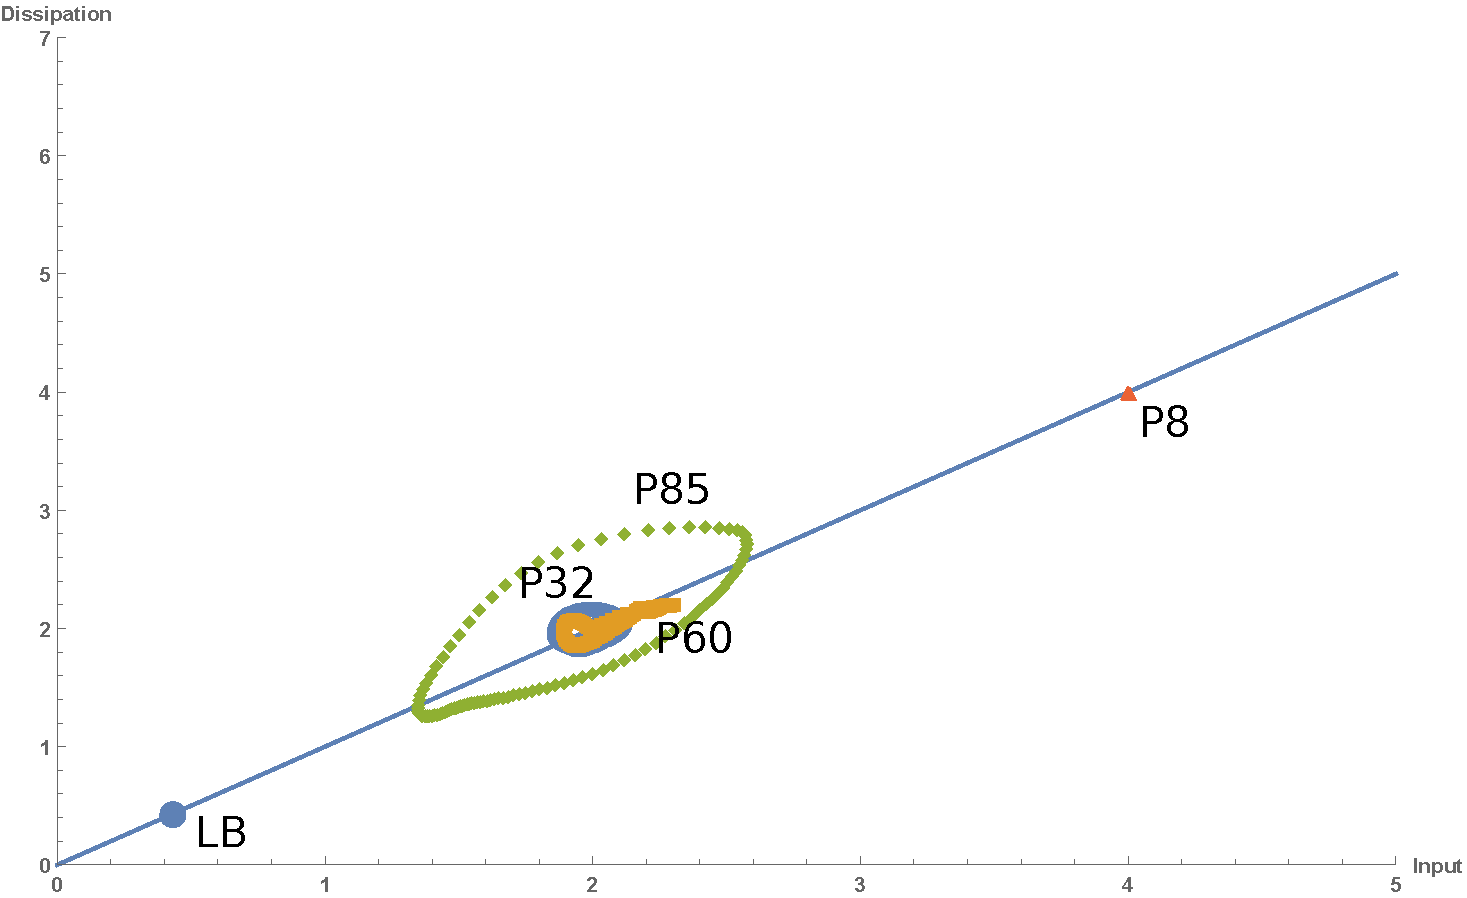
\includegraphics[width=\textwidth]{DIOG}
\caption{DI projection of the Gang of Four, the Nagata lower branch equilibirum (LB), and the line of equal DI. The separation observed in \refFig{fig:POStateSpace} is clearly reflected in this physically important projection.}\label{fig:DIGOF}
\end{figure}

\begin{figure}[h]
\includegraphics[width=\textwidth]{DearGodWhy}
\caption{DI plane projection of 20 turbulent trajectories (red and blue) beginning from random initial conditions, with perturbations of magnitude $0.3$ overlaid on the Gang of Four, the Nagata lower branch equilibrium, and the line of equal DI. Note the separation between P8 and the rest of the Gang of Four.}\label{fig:turbDI}
\end{figure}

\subsection{The Search for Bifurcations, Part II}
The DI projection has another extremely important benefit -- it is domain-agnostic. This allows us to compare the different branches of \refFig{fig:LZBif} in a more sophisticated manner. Since the full bifurcation diagram spans a vast distance in the dissipation-energy input plane, the projection is divided into three parts, with the upper branch in \refFig{fig:DIUpper}, the transition branch in \refFig{fig:DITrans} and the lower branch in \refFig{fig:DILower}, where the divisions between branches is informed by \refFig{fig:LZBif}. In \refFig{fig:DIUpper}, the HKW solution was initially moved up to a higher DI as $L_z$ decreased. However, for finite \ReN, there is a maximum velocity gradient that can be maintained, so the energy input is necessarily bounded, and the orbits begin moving down the DI line, eventually becoming the transition branch. While we were hoping to see an especially meaningful change in the orbit topology at this point, there does not seem to be a great deal of change in its general structure during any bifurcation. In \refFig{fig:DITrans}, the transition branch moves steadily towards the origin of the DI plane.As it does so, its area contracts to a near point, and expands again, eventually becoming the lower branch. The lower branch, in \refFig{fig:DILower} is even less eventful than the transition branch, and generally maintains its structure through its descent towards the origin of the DI plane. Eventually, it reaches the point where \refAlg{alg:parCont} fails, and the continuation process halts.\\
 

\begin{figure}[h]
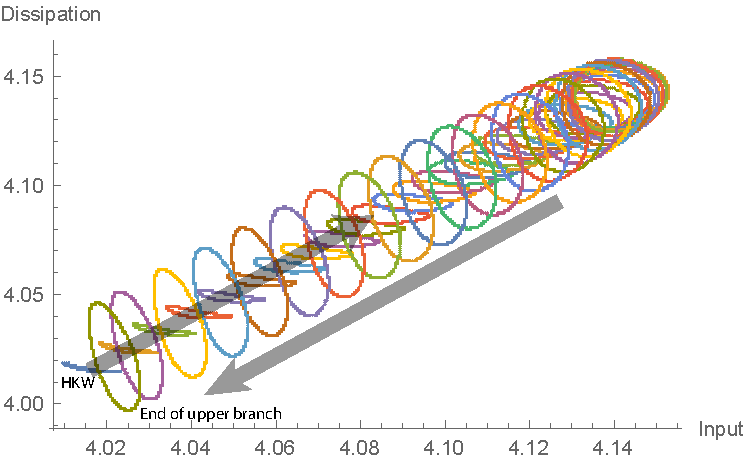
\includegraphics[width=\textwidth]{DIUpper}
\caption{DI plane projection of the upper branch of P8. The HKW solution is the thin blue solution that is continued up to higher DI.}\label{fig:DIUpper}
\end{figure}

\begin{figure}[h]
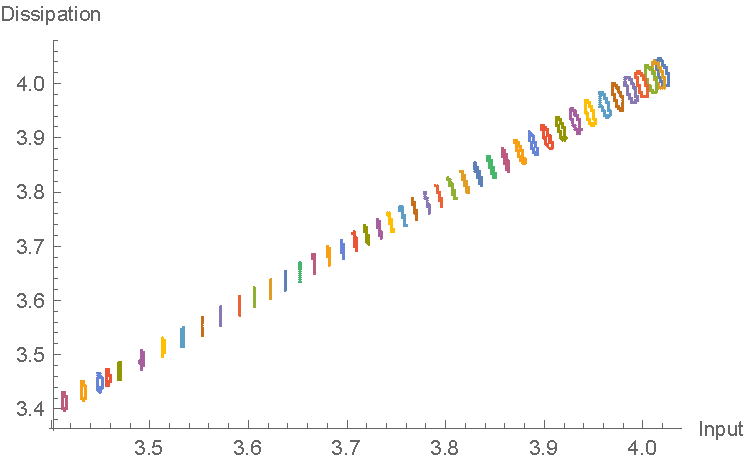
\includegraphics[width=\textwidth]{DITrans}
\caption{The transition branch, which continues to move down the DI line.  }\label{fig:DITrans}
\end{figure}

\begin{figure}[h]
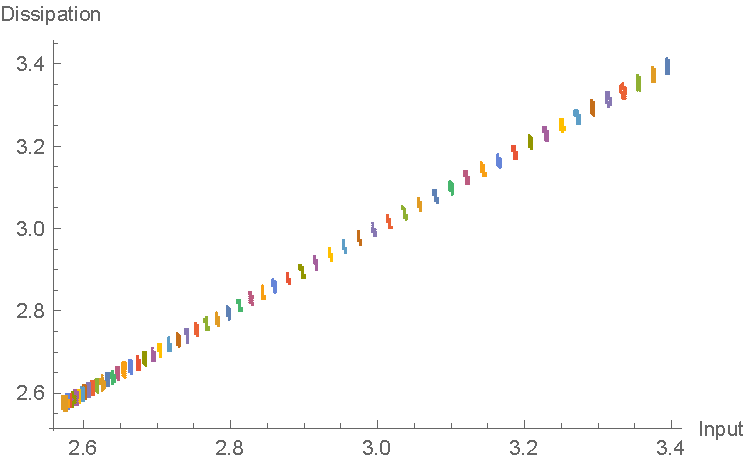
\includegraphics[width=\textwidth]{DILower}
\caption{The lower branch, which moves down the DI line in a similar manner to the transition branch.}\label{fig:DILower}
\end{figure}

However, a glance at \refFigss{fig:DIUpper}{fig:DITrans}{fig:DILower} indicates that the P8s are by and large elliptical in shape, so the area enclosed by the orbit can easily be calculated by the singular value decomposition. Applying this method and ordering by traversal down the continuation trajectory gives \refFig{fig:areaOrder}. Here, the area function begins looking very smooth and Gaussian, but acquires a kink on its way down, after which it behaves in a more complex manner. The fact that the area in the DI plane goes very low is interesting, but probably not indicative of any behavior that has a global effect. Ordering instead by $L_z$ gives \refFig{fig:areaCell}. When the approximate area of P8 is ordered by $L_z$, the features observed in \refFig{fig:areaOrder} take on more meaning. The kink observed in the downwards slope of the Gaussian coincides almost perfectly with the first turning point of \refFig{fig:LZBif}, and the third peak corresponds to the second turning point. While not conclusive, this does show that the turning points are associated with (admittedly slight) structural changes in a physically important projection.  We can also easily calculate the circumference of each orbit by summing the distance between each individual point over the orbit, and obtain \refFig{fig:circumCell}. The similarly to \refFig{fig:LZBif} is noticeable, and is not as trivial as it may sound -- for example a periodic orbit with a small circumference could have a very low velocity, so that it could have a much higher period, so the period and circumference do not necessarily have a linear relationship. \\

\begin{figure}[h!]
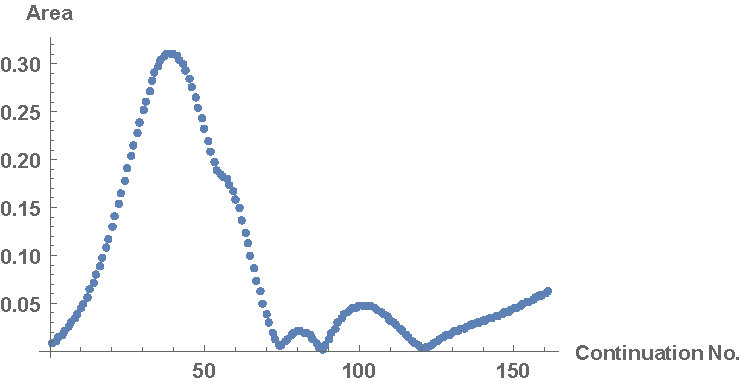
\includegraphics[width=\textwidth]{areaOrder}
\caption{Approximate area of P8 at various $L_z$. Here, the orbits are ordered by traversing \refFig{fig:LZBif}, beginning from the start of the upper branch.}\label{fig:areaOrder}
\end{figure}

\begin{figure}[h!]
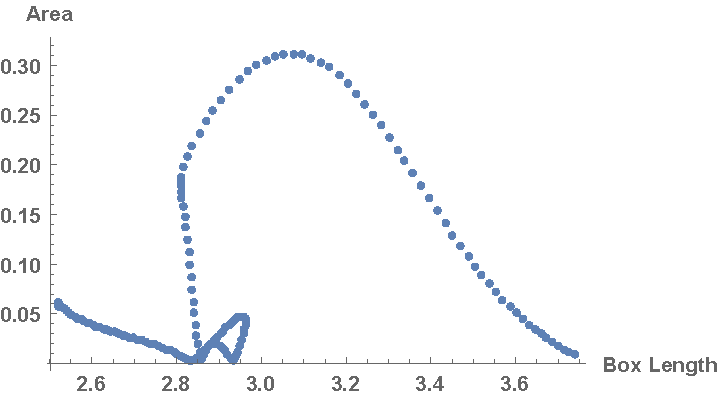
\includegraphics[width=\textwidth]{areaCell}
\caption{Approximate area of P8 at ordered by their $L_z$ values.}\label{fig:areaCell}
\end{figure}

\begin{figure}[h!]
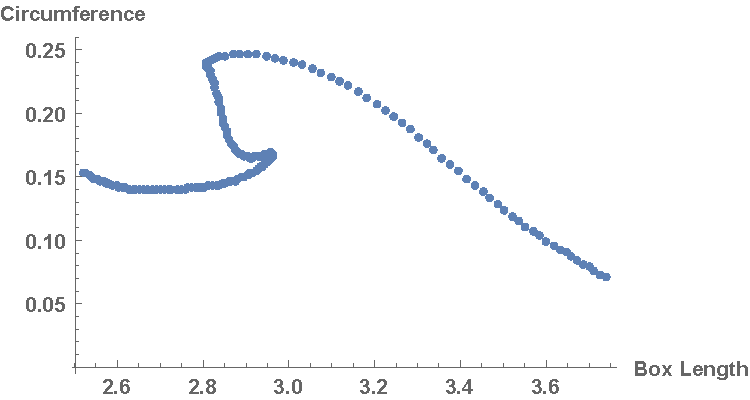
\includegraphics[width=\textwidth]{circumCell}
\caption{The circumference of P8 as a function of $L_z$.}\label{fig:circumCell}
\end{figure}

\clearpage 
This ends the analysis of the Gang of Four, and of P8 in particular (though not for lack of material to analyze...). We will now conclude this thesis by giving a quick summary of the key points, discussing the results, and suggesting potential areas of future research. 